\section{Cualitativas}
En esta sección se abordarán las variables cualitativas, que son aquellas que describen
características o atributos de los elementos de estudio. Estas variables no tienen
un valor numérico intrínseco y se dividen en dos subcategorías principales: nominales y ordinales.
Cómo por sí solas no permiten realizar un análisis estadístico profundo, nos limitaremos a contar la
cantidad de elementos que pertenecen a cada categoría y encontrar la moda, que es la categoría con
mayor frecuencia.

\subsection{Nominales}
En el análisis vamos a trabajar con \Variable{'gender'}.

\TablaDeDatos
\begin{TablaDatosFlexible}
  {
    L{0.24\linewidth}
    C{0.11\linewidth}
    C{0.11\linewidth}
    C{0.11\linewidth}
    C{0.11\linewidth}
  }
  {
    \textbf{Variable} &
    \textbf{fi} &
    \textbf{fr} &
    \textbf{Fi} &
    \textbf{Fr}
  }

\TablaFilaFlexible{\TablaClave{male} & 53 & 47,75\% & 53 & 47,75\%}
\TablaFilaFlexible{\TablaClave{female} & 58 & 52,25\% & 111 & 100,00\%}
\TablaFilaFlexible{\TablaClave{Total} & 111 & 100,00\% & 111 & 100,00\%}

\end{TablaDatosFlexible}

\AnalisisDescriptivo
\PalabraClave{Moda}: female (58 apariciones, 52,3\%) 

\TituloGrafico{male vs female}
\begin{figure}[H]
    \centering
    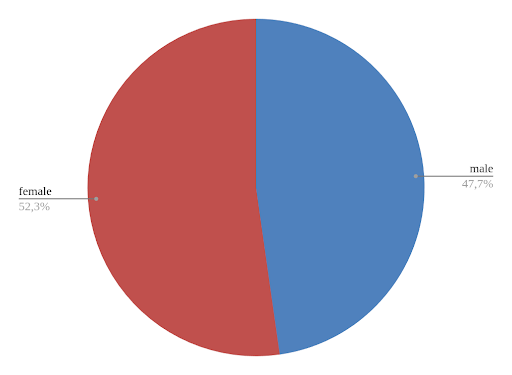
\includegraphics[width=0.7\textwidth]{img/grafico_gender.png}
    \caption{Gráfico de torta para la variable \Variable{gender}.}
    \label{fig:grafico_gender}
\end{figure}

% --------------------------------------------------------------------------------------------------

\subsection{Ordinales}
Ahora vamos a trabajar con \Variable{'parent\_max\_education'}.

\TablaDeDatos
\begin{TablaDatosFlexible}
  {
    L{0.24\linewidth}
    C{0.11\linewidth}
    C{0.11\linewidth}
    C{0.11\linewidth}
    C{0.11\linewidth}
  }
  {
    \textbf{Variable} &
    \textbf{fi} &
    \textbf{fr} &
    \textbf{Fi} &
    \textbf{Fr}
  }

\TablaFilaFlexible{\TablaClave{bachelor\_degree} & 104 & 93,69\% & 104 & 93,69\%}
\TablaFilaFlexible{\TablaClave{master\_degree} & 7 & 6,31\% & 111 & 100,00\%}
\TablaFilaFlexible{\TablaClave{Total} & 111 & 100,00\% & 111 & 100,00\%}

\end{TablaDatosFlexible}

\AnalisisDescriptivo
\PalabraClave{Moda}: bachelor\_degree (104 apariciones, 93,69\%)

\TituloGrafico{Nivel educativo}
\begin{figure}[H]
    \centering
    \includegraphics[width=0.7\textwidth]{img/grafico\_nivel\_educativo.png}
    \caption{Gráfico de barras para la variable \Variable{parent\_max\_education}.}
    \label{fig:grafico_parent_max_education}
\end{figure}
